%\chapter{Image Classification and Convolutional Neural Networks}\label{chap:introCNN}
In this chapter, we will give some basic introduction for supervised 
learning especially for image classification problems. 
Then, we will introduce and define the data and feature space
with related mappings such as convolution and pooling.
In addition, we use the  piecewise (bi-)linear functions on multilevel grids to
interpret the multi-resolution images in the process of CNN. At last, 
we define some classical CNN models mathematically with those notation. 


\section{Supervised learning on image classification}\label{sec:MLbasics}
We consider a basic machine learning problem for classifying a
collection of images into $\kappa$ distinctive classes.  As an
example, we consider a two-dimensional image which is usually
represented by a tensor
$$
f\in \mathbb  \FC := \mathbb{R}^{m\times n\times c}.
$$
Here 
\begin{equation}
\label{data-c}
c=
\left\{
\begin{array}[rl]{rl}
1 & \mbox{for black-white image}\\    
3 & \mbox{for color image}.
\end{array}
\right.
\end{equation}

A typical supervised machine learning problem begins with a data set (training data)
$$
D := \{(f_i, y_i)\}_{i=1}^N,
$$ 
with
$$
\{f_i\}_{i=1}^N \subset \FC,
$$
and $y_i \in \mathbb{R}^{\kappa}$ is the label for data $f_i$, with
$[y_i]_j$ as the probability for $f_i$ in classes $j$. 


Roughly speaking, a supervised learning problem can be thought as data fitting
problem in a high dimensional space $\FC$.
Namely, we need to find a mapping
$$
\classmap:  \mathbb R^{m\times n\times c}\mapsto \mathbb R^\kappa
$$
such that, for a given $f\in  \FC$, 
\begin{equation}\label{eq:idealouput}
\classmap(f)\approx e_i\in \mathbb R^\kappa
\end{equation}
if $f$ is in class $i$, for $1\le i\le \kappa$. 
For the general setting above, we use a probatilistic model for understanding the
output $\classmap(f) \in \mathbb{R}^{\kappa}$ as a discrete 
distribution on $\{1, \cdots,\kappa\}$, with $[\classmap (f)]_i$ as the probability
for $f$ in the class $i$, namely
\begin{equation}
\label{distrib}
0 \le [\classmap(f)]_i \le 1,\quad 
\sum_{i=1}^\kappa  [\classmap(f)]_i=1. 
\end{equation}
At last, we finish our model with a simple strategy to choose
\begin{equation}\label{eq:maxchoose}
\mathop{\arg\max}_{i}\{[\classmap(f)]_i~:~ i = 1:\kappa\},
\end{equation}
as the label for a test data $f$, which ideally is close to
\eqref{eq:idealouput}.  The remaining key issue is the construction of
the classification mapping $\classmap$.


%\subsection{Model construction}
%In many CNN type models for image classification, there are usually
%three major steps to construct $\classmap$.
The main step in the construction of $\classmap$ is to 
construct a nonlinear mapping
\begin{equation}
\label{linearize}
\linearize: \FC \mapsto V_J
\end{equation}
with 
%\begin{equation}
%  \label{F}
%\FC= \mathbb R^{m\times n\times c}  
%\end{equation}
\begin{equation}
\label{VJ}
V_J = \mathbb R^{m_J\times n_J\times c_J}. 
\end{equation}
To be consistent with the notation for CNN which will be described below,
here the subscript $J$ refers to the number of 
coarsening girds in CNN. 
Roughly speaking, the map $\linearize$ plays two roles.  The first role
is to make a dimension reduction, namely
$$
m_Jn_Jc_J\ll  mnc.
$$
The second role is to map a complicated set of data into a set of data
that are linearly separable. As a result, the simple logistic regression 
procedure can be applied.

The first step in a logistic regression it to introduce a linear mapping:
\begin{equation*}
\Theta: \FC \to\mathbb{R}^{\kappa} ,
\end{equation*}as 
\begin{equation}\label{thetamap}
\Theta(x)=Wx+b,
\end{equation}
where $W=(w_{ij})\in\mathbb{R}^{(m_J \times n_J \times c_J)\times \kappa}$, 
$b\in\mathbb{R}^{\kappa}$.


We then use the soft-max function.
\begin{equation}
\label{softmax}
[S(z)]_i=[{\rm Solftmax}(z)]_i= \frac{e^{z_i}}{\sum_{j} e^{z_j}},
\end{equation}
to obtain a logistic regression model 
\begin{equation}
\label{eq:log_reg}
S \circ \Theta: \mathbb R^{m_J\times n_J\times c_J}\mapsto \mathbb R^\kappa.
\end{equation}
%	This makes $S\circ \linearize(f) \in \mathbb{R}^\kappa$ as a distribution on 
%	$\{1,\cdots,\kappa\}$. 

By combining the nonlinear mapping $\classmap$ in \eqref{linearize}
and the logistic regression \eqref{eq:log_reg}, we obtain the following classifier:
\begin{equation}
\label{classifier}
\classmap=  S\circ \Theta\circ \linearize.
\end{equation}

%\subsection{Loss function and training}  
Given the model \eqref{classifier},
we finish the training phase with solving the next optimization 
problem:
\begin{equation}
\label{eq:abstractloss}
\min \sum_{j=1}^Nl(\classmap(f_j),y_j),
\end{equation}
where
Here $l(\classmap(f_j),y_j)$ is a  loss function that measures the
predicted result $\classmap(f_j)$ and the real label $y_j$. 
In logistic regression, 
the following cross-entropy loss function is often used
\begin{equation}\label{eq:cross-entropy}
l(\classmap(f), y) = \sum_{i=1}^\kappa -[y]_i \log [\classmap(f)]_i.
\end{equation}

\section{Data space, feature space and relevant mappings}\label{sec:spaces}
Given a data
\begin{equation}
\label{data-f}
f \in \mathbb{R}^{m \times n \times c}, 
\quad \text{or}\quad [f]_i \in
\mathbb{R}^{m\times n}, \quad i = 1:c,
\end{equation}
where $m\times n$ is called the spatial dimension and $c$ is the 
channel dimension.

For the given data $f$ in \eqref{data-f}, we look for some
feature vector, denoted by $u$,  associated with $f$:
\begin{equation}
\label{u}
u \in \mathbb{R}^{m \times n \times h}.
\end{equation}
We make an assumption that the data $f$ and feature $u$ are related by a mapping 
(which can be either linear or nonlinear)
\begin{equation}
\label{u}
A:  \mathbb{R}^{m \times n \times h}\mapsto \mathbb{R}^{m \times n \times c}, 
\end{equation}
so that
\begin{equation}
\label{Auf}
A(u)=f. 
\end{equation}
A mapping 
\begin{equation*}
B : \mathbb{R}^{m\times n\times c} \mapsto \mathbb{R}^{m \times n\times h},
\end{equation*}
is called a feature extractor if $B \approx A^{-1}$ and 
\begin{equation}\label{vBf}
v = B(f),
\end{equation}
is such that $v \approx u$.

The data-feature relationship \eqref{Auf} or \eqref{vBf} is not
unique.   Different relationships give rise to different features. 
We can view the data-feature relationship given in \eqref{Auf}
as a model that we propose.  Here the mapping $A$, which can be either
linear or nonlinear, is unknown and needs to be trained.  

%\begin{remark}
We point out  that the data space and feature space may have different
numbers of channels.
%\end{remark}

\subsection{A special linear mapping: convolution}
%Firstly, as mentioned before, an image type
%data with multichannel can be understand as  
%vector valued functions
%$$
%f \in \mathbb{R}^{m \times n \times c}, \quad \text{or}\quad [f]_i \in
%\mathbb{R}^{m\times n}, \quad i = 1:c,
%$$
One important class of linear mapping is the so called convolution:
%We first consider $\theta$ a convolution operator (with stride $1$) 
%and padding:
$$
\theta: \mathbb{R}^{m\times n\times c} \mapsto \mathbb{R}^{m\times n \times h},
$$
that can be defined by 
\begin{equation}\label{conv-1}
[\theta(f)]_{t} = \sum_i^{c}K_{i,t} \ast [f]_i + b_t 
\bm{1}  \in \mathbb{R}^{m\times n}, \quad t = 1:h,
\end{equation}
where $\bm{1}  \in \mathbb{R}^{m\times n} $ is a 
$m\times n$ matrix with all elements being $1$,
and for $g \in \mathbb{R}^{m\times n}$
\begin{equation}\label{con1}
[K \ast g]_{i,j} = \sum_{p,q=-k}^k K_{k+1+p,k+1+q} g_{i + p, j + q}, \quad i=1:m, j = 1:n.
\end{equation}
The coefficients in \eqref{con1} constitute  a kernel matrix
\begin{equation}
K \in \mathbb{R}^{(2k+1) \times (2k+1)},
\end{equation}
where $k$ is often taken as small integers. 
Here padding means how choose $ X_{i+ p, j + q}$ 
when $(i+ p, j + q)$ is out of $1:m$ or $1:n$. 
Those next three choices are often used
\begin{equation}\label{eq:padding}
f_{i + p, j + q} = \begin{cases}
0,  \quad &\text{zero padding}, \\
f_{(i + p)\pmod{m}, (s + q)\pmod{n}},  \quad &\text{periodic padding}, \\
f_{|i-1 +p|, |j -1  +q|},  \quad &\text{reflected padding}, \\
\end{cases}
\end{equation}
if 
\begin{equation}
i + p \notin \{1, 2, \dots, m\} ~\text{or} ~  j+ q \notin \{1, 2, \dots, n\}.
\end{equation}
Here $ d \pmod m \in \{1, \cdots, m\} $  means the remainder when $d$ is divided by $m$.

%Then we remark that, if we take convolution without pooling, there is a 
%shift with 
%$$
%i+ p  \rightarrow i + k+ p,
%$$
%and also for $j$ such that all index $(i + k+ p, j + k+ p)$ is during
%$1:n$. 

If we formally write 
\begin{equation}
f=
\begin{pmatrix}
f_1\\
\vdots\\
f_c  
\end{pmatrix}
\end{equation}
We can then write the operation \eqref{conv-1} as
\begin{equation}
\label{eq:4}
\theta(f)=K\ast f+b
\end{equation}
where 
$$
K=(K_{ij})\in \mathbb R^{[(2k+1)\times(2k+1)]\times h\times c}
$$
and 
$$
\bm{b}=\bm{1}_{m\times n}\otimes b.
$$

The operation \eqref{eq:4} is also called a convolution with stride 1. More generally, 
given an integer $s\ge1$, a convolution with stride $s$ for $f \in \mathbb{R}^{m\times
	n}$ is defined as:
\begin{equation}\label{stride}
[K \ast_s f]_{i,j} = \sum_{p,q=-k}^k K_{p,q} f_{s(i-1)+1 + p, s(j-1)+1 + q},  
\quad i = 1: \lceil  \frac{m}{s}\rceil , j = 1: \lceil  \frac{n}{s}\rceil.
\end{equation}
Here $ \lceil  \frac{m}{s}\rceil$ denotes the smallest integer that greater than $\frac{m}{s}$.
In CNN, we often take $s=2$.


\subsection{Some linear and nonlinear mappings and extractors}
A data-feature map $A$ and feacture extractor $B$ can be either
linear or nonlinear.   The nonlinearity can be obtained from
appropriate application of an activation function
\begin{equation}
\label{act}
\sigma: \mathbb{R} \to \mathbb{R} .
\end{equation}
In this paper, we mainly consider a special activation function, known 
as the {\it rectified linear unit} (ReLU), which is defined by
\begin{equation}
\label{relu}
\sigma(x)= {\rm ReLU}(x) :=\max(0,x), \quad x\in\mathbb{R}. 
\end{equation}
By applying the function to each component, we can extend this
\begin{equation}
\label{vector-act}
\sigma:\mathbb R^{m\times n\times c}\mapsto \mathbb R^{m\times n\times c}.  
\end{equation}


A linear data-feature mapping can simply given by a convolution as in \eqref{con1}:
\begin{equation}
\label{linearA}
A(f)=\xi\ast f
\end{equation}
A nonlinear mapping can be given by compositions of convolution and
activation functions:
\begin{equation}
\label{nonlinearA}
A=\xi\circ\sigma\circ\eta ,
\end{equation}

and 
\begin{equation}
\label{extractor}
B=\sigma\circ \gamma \circ\sigma  .
\end{equation}
Here $\xi$, $\eta$ and $\gamma$ are all 
appropriate convolution mappings.


\subsection{An iterative feacture extraction scheme}
One key idea in this paper is that we use a simple iterative
process to approximately solve \eqref{Auf} using \eqref{vBf}. Namely,
for $i=1:\nu$
\begin{equation}\label{eq:smoothB}
u^{i} = u^{i-1} + B^{i}(f- A(u^{i-1})) 
\end{equation}
for an appropriately chosen $u^0$.  We refer to \cite{xu1992iterative}
for more discussion on iterative scheme in the form of \eqref{eq:smoothB}.



\section{Piecewise (bi-)linear functions on multilevel grids}\label{sec:functions}
An image can be viewed as a function on a grid.  Images
with different resolutions can then be viewed as functions on grids of
different sizes.  The use of such multiple-grids is a main technique
used in the standard multigrid method for solving discretized partial
differential equations \cite{xu1992iterative, xu2002method}, 
and it can also be interpreted as a main ingredient used in
convolutional neural networks (CNN). 

Without loss of generality, for simplicity, we assume that the initial
grid, $\mathcal T$, is of size
$$
m=2^{s}+1, n=2^{t}+1 
$$
for some integers $s, t\ge 1$.
Starting from $\mathcal T_1=\mathcal T$,  we consider a sequence of
coarse grids (as depicted in Fig.~\ref{mgrid} with $J=4$):
\begin{equation}
\label{grids}
\mathcal T_1, \mathcal T_2, \ldots, \mathcal T_J
\end{equation}
such that ${\mathcal T}_\ell$ consist of $m_\ell\times n_\ell$ grid
points, with 
\begin{equation}
\label{mn-ell}
m_\ell=2^{s-\ell+1}+1, n_\ell=2^{t-\ell+1}+1.   
\end{equation}
\begin{figure}[!htbp]\label{mgrid}
	\begin{center}
		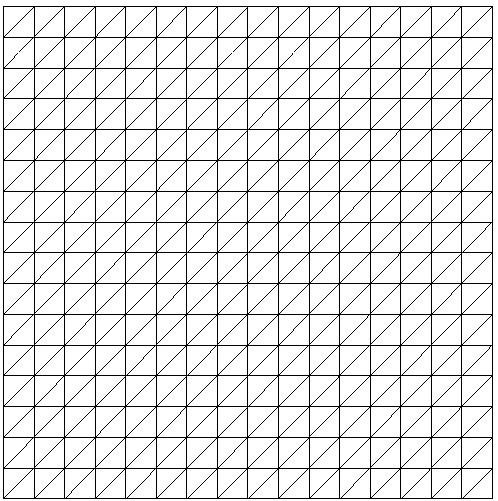
\includegraphics[width=0.15\textwidth]{grid2.png} \quad 
		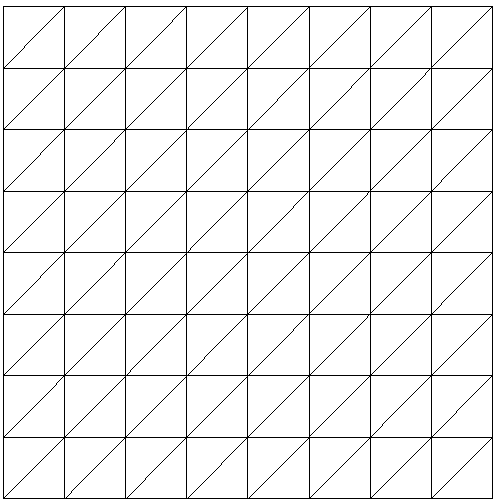
\includegraphics[width=0.15\textwidth]{grid1.png} \quad 
		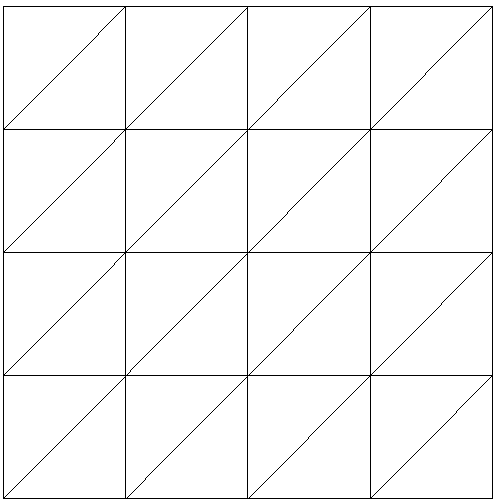
\includegraphics[width=0.15\textwidth]{grid0.png} \quad 
		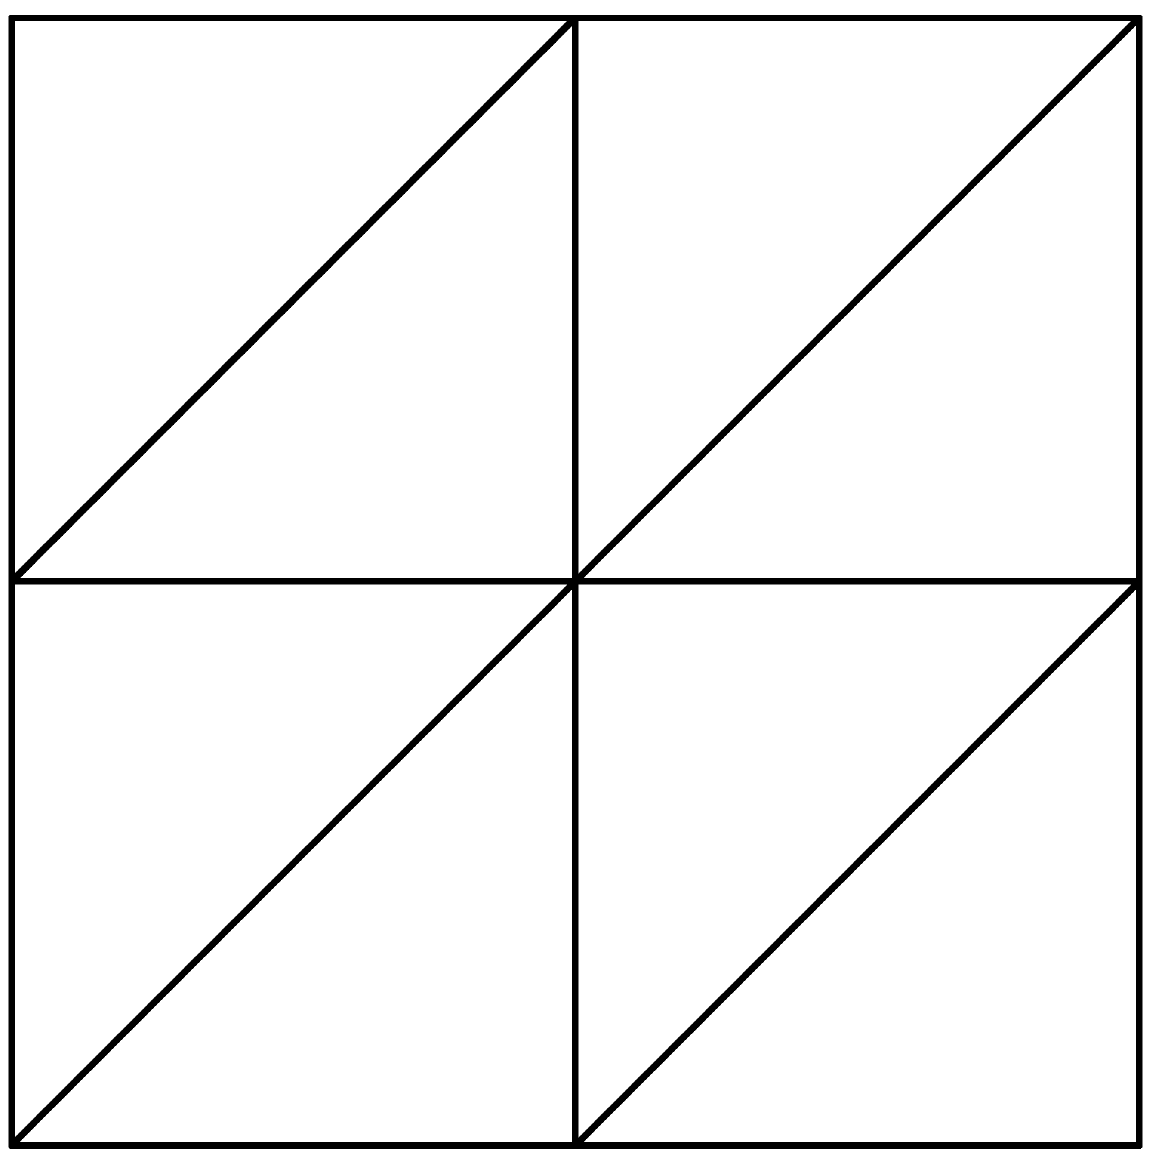
\includegraphics[width=0.15\textwidth]{grid.png} 
	\end{center}
	$$ 
	\mathcal T_1\hskip1in \mathcal T_2\hskip1in \mathcal T_3\hskip1in\mathcal T_4
	$$
	\caption{multilevel grids for piecewise linear functions}
\end{figure}

The grid points of these grids can be given by
$$
x_i^{\ell}=i h_{1,\ell}, y_j^{\ell}=j h_{2,\ell},  i=1, \ldots, m_\ell,
j=1, \ldots, n_\ell.
$$
Here $h_{1,\ell} = 2^{-s + \ell -1}a$ and $h_{2,\ell} = 2^{-t + \ell - 1}b$,
for some $a,b >0$. The above geometric coordinates $(x_i^\ell, y_i^\ell)$
are usually not used in image precess literatures, but they are relevant
in the context of multigrid method for numerical solution of PDEs.
We now consider piecewise linear functions on the sequence of grids
\eqref{grids} and we obtain a nested sequence of linear vector spaces
\begin{equation}
\label{Vk}
\mathcal V_1\supset\mathcal V_2\supset\ldots\supset \mathcal
V_J.
\end{equation}
Here each $\mathcal V_\ell$ consists of all piecewise bilinear (or linear)
functions with respect to the grid \eqref{grids} and \eqref{mn-ell}.
Each $\mathcal V_\ell $ has a set of basis functions:
$\phi_{ij}^\ell\in \mathcal V_\ell$ satisfying:
$$
\phi_{ij}^\ell(x_p,y_q)=\delta_{(i,j), (p,q)} = 
\begin{cases}
1 \quad &\text{if} \quad (p,q) = (i,j), \\
0 \quad &{\text{if}} \quad (p,q)\neq (i,j).
\end{cases}
$$
Thus, for each $v \in \mathcal V_{\ell}$, we have 
\begin{equation}\label{expand}
v(x,y)=\sum_{i,j}v^\ell_{ij}\phi_{ij}^\ell(x,y).
\end{equation}
\subsection{Prolongation}
Given a piecewise (bi-)linear function $\bm v\in\mathcal V_{\ell+1}$, the
nodal values of $\bm v$ on $m_{\ell+1}\times n_{\ell+1}$ grids point
constitute a tensor
$$
v^{\ell+1}\in \mathbb R^{m_{\ell+1}\times n_{\ell+1}}.
$$
We note that $\bm v\in\mathcal V_{\ell}$ thanks to \eqref{Vk} and the
nodal values of $\bm v$ on $\mathcal T_\ell$ 
constitute a tensor
$$
v^{\ell}\in \mathbb R^{m_{\ell}\times n_{\ell}}.
$$
Using the property of piecewise (bi-)linear functions, it is easy to see that 
\begin{equation}
\label{eq:13}
v^{\ell}=\bar P_{\ell+1}^\ell v^{\ell+1}  
\end{equation}
where 
\begin{equation}
\label{mg-prolong}
\bar P_{\ell+1}^\ell: \mathbb R^{m_{\ell+1}\times n_{\ell+1}}\mapsto  \mathbb R^{m_{\ell}\times n_{\ell}}  
\end{equation}
which is called a prolongation in multigrid terminology.  More
specifically, 
\begin{equation}
\label{eq:7}
v^{\ell}_{2i-1,2j-1}=  v^{\ell+1}_{i,j},
\end{equation}
with 
\begin{equation}
\label{eq:9}
v^{\ell}_{2i-1, 2j} = \frac{1}{2}(v^{\ell+1}_{i,j} + v^{\ell+1}_{i,j+1}), \quad 
v^{\ell}_{2i, 2j-1} = \frac{1}{2}(v^{\ell+1}_{i,j} + v^{\ell+1}_{i+1,j}),
\end{equation}
and
\begin{equation}
%\begin{tiny}
%{\scriptsize 
v^{\ell}_{2i, 2j}  =  
\begin{cases}
\frac{1}{4}(v^{\ell+1}_{i,j} + v^{\ell+1}_{i+1,j} + v^{\ell+1}_{i,j+1} + v^{\ell+1}_{i+1,j+1}),  &\text{if $v^\ell$ is piecewise bilinear }, \\
\frac{1}{2}( v^{\ell+1}_{i+1,j} + v^{\ell+1}_{i,j+1}), &\text{if $v^\ell$ is piecewise linear }.
\end{cases}
%\end{tiny}
%}
\end{equation}
%when
%\begin{description}
%\item[$v^\ell$ is piecewise bilinear] 
%\begin{equation}
%\label{eq:pro-bilinear}
%v^{\ell}_{2i, 2j} = \frac{1}{4}(v^{\ell+1}_{i,j} + v^{\ell+1}_{i+1,j} + v^{\ell+1}_{i,j+1} + v^{\ell+1}_{i+1,j+1}),
%\end{equation}
%\item[$v^\ell$ is piecewise linear] 
%\begin{equation}
%\label{eq:pro-linear}
%v^{\ell}_{2i, 2j} = \frac{1}{2}( v^{\ell+1}_{i+1,j} + v^{\ell+1}_{i,j+1}).
%\end{equation}
%\end{description}

\subsection{Pooling, restriction and interpolation}\label{sec:cnn-restriction}
The prolongation given by \eqref{mg-prolong} can be used to transfer
feature from a coarse grid to a fine grid.   
On the other hand, we also
need a mapping, known as restriction,  that transfer data from fine grid to corse grid:
\begin{equation}
\label{mg-restrict}
\bar R_\ell^{\ell+1}: \mathbb R^{m_{\ell}\times n_{\ell}}  \mapsto  \mathbb R^{m_{\ell+1}\times n_{\ell+1}}.
\end{equation}
%This operation can often be obtained by two different steps. 
%First, we carry out a convolution operation $\tilde R: \mathbb R^{n_\ell\times n_\ell}\mapsto 
%\mathbb R^{n_\ell\times n_\ell}$:
%\begin{equation}
%\label{linear-restriction}
%\begin{aligned}
%(\tilde Rr)_{i,j}&=r_{i,j} +{1\over 2}(r_{i,j-1} + r_{i,j+1} + r_{i-1,j} + r_{i+1,j} + r_{i+1,j-1} + r_{i-1,j+1}) ,
%\end{aligned}
%\end{equation}
%Then, we define
%\begin{equation}
%\label{linear-restriction-stride}
%(Rr)_{i,j}=(\tilde R r)_{2i-1,2j-1}, \quad 1\le i, j \le n_{\ell+1}.
%\end{equation}
%%Using the terminology from deep learning \cite{goodfellow2017deep}, 
%As the definition in above section,
%we note that \eqref{linear-restriction} and \eqref{linear-restriction-stride} can be written as a
%convolution with a $3\times3$ kernel with stride 2:
%\begin{equation}\label{eq:restriction}
%Rr=K\ast_2 r,\quad K=\left ( \begin{array}{ccc}
%0 &\frac{1}{2}&\frac{1}{2}\\
%\frac{1}{2}& 1&\frac{1}{2}\\
%\frac{1}{2}&\frac{1}{2}& 0
%\end{array}\right ).
%\end{equation}
In multigrid for solving discretized partial differential equation,
the restriction is often taken to be transpose of the prolongation
given by \eqref{mg-prolong}:
\begin{equation}
\label{mg-RP}
\bar R_\ell^{\ell+1} = [\bar P_{\ell+1}^\ell]^T.  
\end{equation}
\begin{lemma}
	If $\tilde P_{\ell+1}^\ell$ takes the form of prolongation
	in multigrid methods for linear finite element functions 
	on the above grids, then $\tilde R_{\ell}^{\ell+1}$ is 
	a convolution with stride $2$ and a $3\times3$
	kernel as:
	\begin{equation}\label{restriction}
	R_\ell^{\ell+1} f=K_R\ast_2 f,
	\end{equation} 
	where, if $\mathcal V_\ell$ is piecewise bilinears, 
	\begin{equation}\label{bi-restrict}
	K_R=
	\begin{pmatrix}
	\frac{1}{4} &\frac{1}{2}&\frac{1}{4}\\
	\frac{1}{2}& 1&\frac{1}{2}\\
	\frac{1}{4}&\frac{1}{2}&  \frac{1}{4} 
	\end{pmatrix},
	\end{equation}
	or, if $\mathcal V_\ell$ is piecewise linears, 
	\begin{equation}
	\label{linear-restrict}
	K_R=
	\begin{pmatrix}
	0 &\frac{1}{2}&\frac{1}{2}\\
	\frac{1}{2}& 1&\frac{1}{2}\\
	\frac{1}{2}&\frac{1}{2}&  0
	\end{pmatrix}.
	\end{equation}
\end{lemma} 
In addition, all these convolutions are applied with zero padding as in \eqref{eq:padding}
, which is consistent with the Neumann boundary condition for applying FEM to 
numerical PDEs. More details will be discussed in \S \ref{sec:cnn-restriction}.

In the deep learning literature, the restriction such as
\eqref{mg-restrict} is often known as pooling operation.  One popular
pooling is a convolution with stride $s$, with some small integer $s>1$.  

Some other fixed (or untrained) poolings are also often used.  
One popular pooling is the so called average pooling $R_{avr}$ which
can be a convolution with stride $2$ or bigger using the  kernel $K$
in the form of
\begin{equation}
\label{average-K}
K=
\frac{1}{9}\begin{pmatrix}
1 & 1 & 1 \\
1 & 1 & 1 \\
1 & 1 & 1
\end{pmatrix}. 
\end{equation}
Nonlinear pooling operator is also used, for the example the $(2k+1)
\times (2k+1)$ max-pooling operator with stride $s$ as follows:
\begin{equation}
[{R}_{\rm max}(f)]_{i,j} = \max_{-k\le p ,q\le k} \{f_{s(i-1)+1 + p, s(j-1)+1 +q} \}.
\end{equation}

Another approach to the construction of restriction of pooling can be 
obtained by using interpolation. 
Given 
$$
v^\ell\in \mathbb \mathbb R^{m_{\ell}\times n_{\ell}}, 
$$
let $\bm v\in \mathcal V_\ell$ be the function whose nodal values are
precisely give by $v^\ell$ as in \eqref{expand}.  
Any reasonable linear operator
\begin{equation}
\label{eq:11}
\Pi:  \mathcal V_\ell\mapsto \mathcal V_{\ell+1},
\end{equation}
such as: 
nodal value interpolation, 
Scott-Zhang interpolation and
$L^2$ projection \cite{xu2019FEM},
would give rise to a mapping
\begin{equation}
\label{mg-Pi}
\Pi_\ell^{\ell+1}: \mathbb R^{m_{\ell}\times n_{\ell}}  \mapsto
\mathbb R^{m_{\ell+1}\times n_{\ell+1}},
\end{equation}
such that
$$
v^{\ell+1}=\Pi_\ell^{\ell+1} v^\ell.
$$
As situations permit, we can use these a priori given restrictions to replace
unknown pooling operators to reduce the number of parameters.





